\section{Dynamic Switching Visualization} \label{switching-visualization}
The configuration switching happens during both phases of the READEX methodology. 
During DTA, PTF runs experiments with different configurations to find the optimal configuration for each rts in the application, which are then stored in the tuning model. 
This requires configuration switching during the application run. 
During RAT, for each rts, the optimal configuration from the tuning model is applied while the application is running which also requires configuration switching.

To enable the user to visualize the configuration switching for each region during DTA and during a production run, a switching visualization module is also included in RRL. 
The visualization module is implemeted as a Score-P Metric Plugin. 
The metric plugin uses the Mertic Plugin Interface provided in Score-P \cite{Schoene2017}. 
Each of the tuning parameters is added as a metric and recorded in an OTF2 \cite{Ilsche-Cstate} trace by Score-P. 
The OTF2 trace generated can be visualized in the Vampir \cite{BHJR:10:VampirOverview}. 
The user can select these metrics in Vampir and visualize the switching pattern for each metric.
The tuning parameters selection is configurable and the user can specify if all the tuning parameters or a subset has to be recorded in OTF2 trace. 
Any of the hardware, software and application tuning parameters can be chosen for visualization.
Figure~\ref{fig:switch_visualization} illustrates the switching of the CPU frequency and uncore frequency performed by
RRL while tuning CPU frequency and uncore frequency for the Blasbench benchmark.
\begin{figure}[!t]
\centering
%\includegraphics[trim={7cm 2cm 5.5cm 2cm},clip,width=3in]{readex-approach}
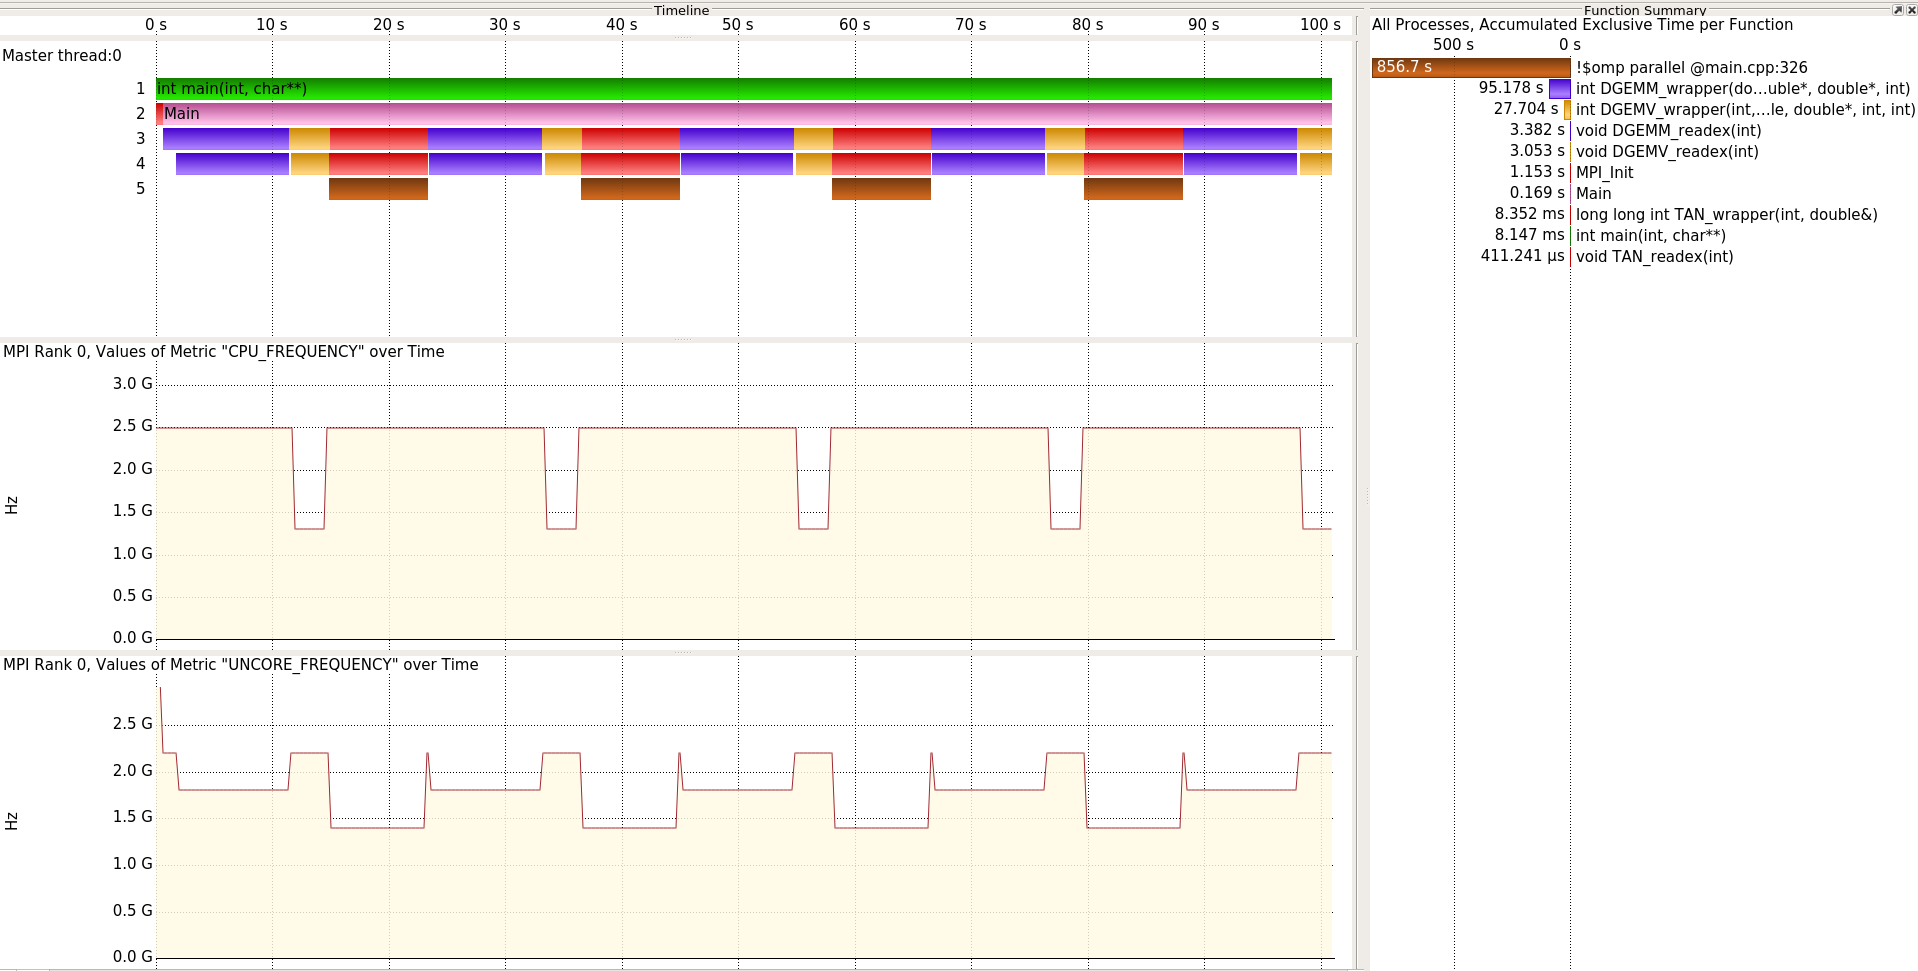
\includegraphics[width=.95\columnwidth]{figures/visualization_trace.png}
\caption{{CPU\_FREQUENCY} and {UNCORE\_FREQUENCY} switchings during Blasbench runtime tuning}
\label{fig:switch_visualization}
\end{figure}

 